%!TEX program = xelatex
\documentclass[a4paper,12pt]{report}
\usepackage{indentfirst} 
\usepackage{ctex}
%\usepackage{xeCJK}
\usepackage{times}
\usepackage{graphicx,float}
\usepackage{subcaption}
\usepackage{setspace}
\usepackage{fancyhdr}
% \usepackage{graphicx}
\usepackage{wrapfig}
\usepackage{array}
\usepackage{fontspec,xunicode,xltxtra}
\usepackage{titlesec}
\usepackage{titletoc}
\usepackage[titletoc]{appendix}
\usepackage[top=30mm,bottom=30mm,left=20mm,right=20mm]{geometry}
\usepackage{cite}
\usepackage{listings}
\usepackage[framed,numbered,autolinebreaks,useliterate]{mcode} % 插入代码
\XeTeXlinebreaklocale "zh"
\XeTeXlinebreakskip = 0pt plus 1pt minus 0.1pt

%---------------------------------------------------------------------
%	页眉页脚设置
%---------------------------------------------------------------------
\fancypagestyle{plain}{
	\pagestyle{fancy}      %改变章节首页页眉
}

\pagestyle{fancy}
\lhead{\kaishu~``计算机网络''实验报告~}
\rhead{\kaishu~~实验3:路由协议}
\cfoot{\thepage}

%---------------------------------------------------------------------
%	章节标题设置
%---------------------------------------------------------------------
\titleformat{\chapter}{\centering\zihao{-1}\heiti}{实验3.\arabic{chapter}}{1em}{}
\titlespacing{\chapter}{0pt}{*0}{*6}

%---------------------------------------------------------------------
%	摘要标题设置
%---------------------------------------------------------------------
\renewcommand{\abstractname}{\zihao{-3} 摘\quad 要}

%---------------------------------------------------------------------
%	参考文献设置
%---------------------------------------------------------------------
\renewcommand{\bibname}{\zihao{2}{\hspace{\fill}参\hspace{0.5em}考\hspace{0.5em}文\hspace{0.5em}献\hspace{\fill}}}

%---------------------------------------------------------------------
%	引用文献设置为上标
%---------------------------------------------------------------------
\makeatletter
\def\@cite#1#2{\textsuperscript{[{#1\if@tempswa , #2\fi}]}}
\makeatother

%---------------------------------------------------------------------
%	目录页设置
%---------------------------------------------------------------------
\titlecontents{chapter}[0em]{\songti\zihao{-4}}{\thecontentslabel\ }{}
{\hspace{.5em}\titlerule*[4pt]{$\cdot$}\contentspage}
\titlecontents{section}[2em]{\vspace{0.1\baselineskip}\songti\zihao{-4}}{\thecontentslabel\ }{}
{\hspace{.5em}\titlerule*[4pt]{$\cdot$}\contentspage}
\titlecontents{subsection}[4em]{\vspace{0.1\baselineskip}\songti\zihao{-4}}{\thecontentslabel\ }{}
{\hspace{.5em}\titlerule*[4pt]{$\cdot$}\contentspage}

\renewcommand\thesection{\arabic{section}}
\renewcommand\thesubsection{\arabic{section}.\arabic{subsection}}
\setcounter{tocdepth}{3}
\setcounter{secnumdepth}{3}
\begin{document}
%---------------------------------------------------------------------
%	封面设置
%---------------------------------------------------------------------
\begin{titlepage}
	\begin{center}
		
    
\includegraphics[width=1.0\textwidth]{figure//nankai.jpg}\\
    % \vspace{10mm}
    % \textbf{\zihao{2}\kaishu{软件学院}}\\[0.8cm]
    \vspace{50mm}
    \textbf{\zihao{1}\heiti{ 《计算机网络》实验报告}}\\[1cm]
    \textbf{\zihao{2}\heiti{ (2022\textasciitilde2023学年第一学期)}}\\[1cm]
    % \textbf{\zihao{3}\heiti{ 实验1: Wireshark 软件使用与ARP 协议分析}}\\[2cm]
	\vspace{\fill}
	
\setlength{\extrarowheight}{2mm}
{\songti\zihao{3}	
\begin{tabular}{rl}

	{\makebox[4\ccwd][s]{实验名称:}}& ~\kaishu 路由协议\\
	{\makebox[4\ccwd][s]{学\qquad 院:}}& ~\kaishu 软件学院\\
		{\makebox[4\ccwd][s]{姓\qquad 名:}}& ~\kaishu 张怡桢\\

    {\makebox[4\ccwd][s]{学\qquad 号:}}& ~\kaishu 2013747 \\

	{\makebox[4\ccwd][s]{指导老师:}} & ~\kaishu 张圣林\\

\end{tabular}
 }\\[2cm]
\vspace{\fill}
\zihao{4}
%2021\textasciitilde 2022秋季学期\\
%使用\LaTeX 撰写于
    \today
	\end{center}	
\end{titlepage}


%---------------------------------------------------------------------
%  目录页
%---------------------------------------------------------------------
\tableofcontents % 生成目录

%---------------------------------------------------------------------
%  实验3.1
%---------------------------------------------------------------------
\chapter{静态路由
}
\setcounter{page}{1}
\begin{spacing}{1.5}
\songti\zihao{-4}

%\section{分工情况}
 %\begin{itemize}
 %	\item 张三:
 %	\item 李四:
 %	\item 六六:
 %\end{itemize}

\section{实验目的}
掌握静态路由协议,理解路由器工作原理,掌握路由器相关的配置、检测操作。

\section{实验内容}
\begin{itemize}
  \item GNS3设备常用配置命令;
  \item 网络模拟器GNS3的安装;
  \item IP 地址的配置;
  \item 静态路由的配置;
  \item 路由规划;
  \item 网络收敛的概念;
  \item 网络测试与排错操作。
\end{itemize}

\section{实验原理、方法和手段}
\begin{figure}[htb!]
  \centering
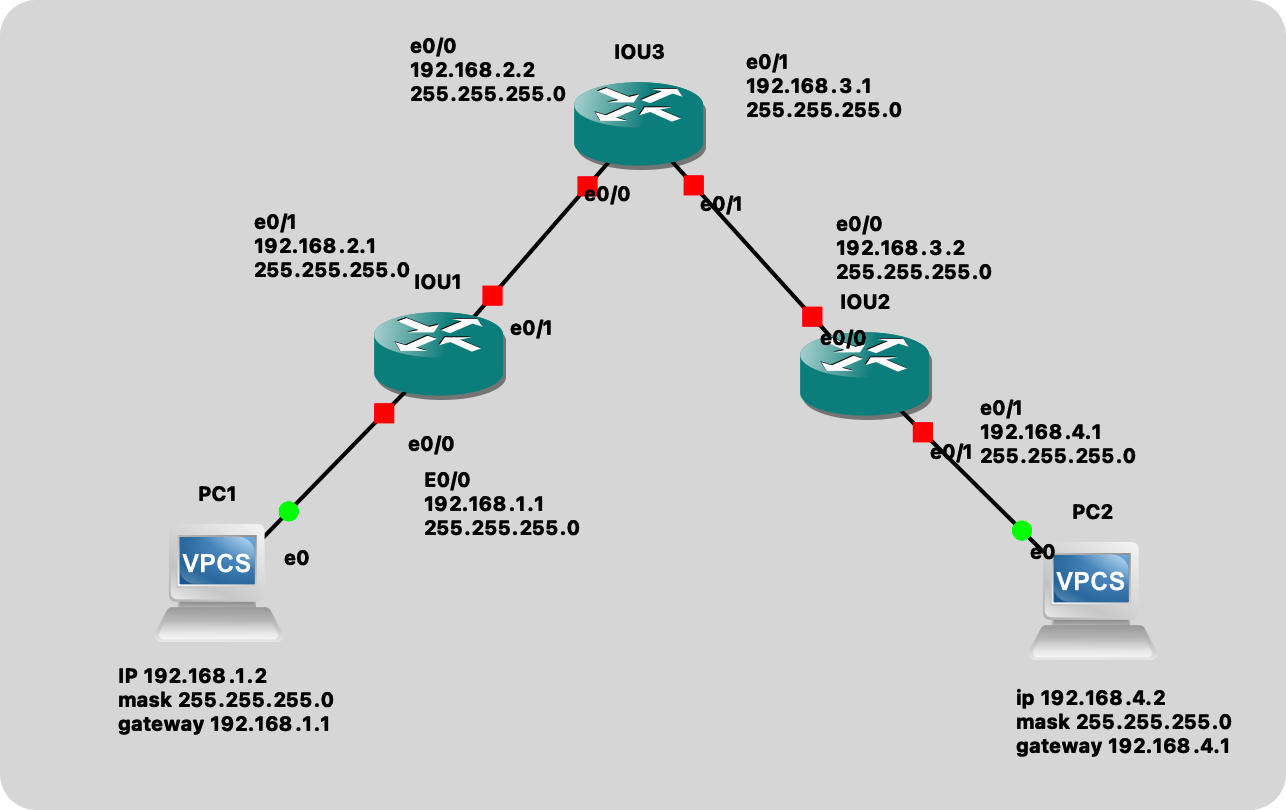
\includegraphics[width=12cm]{figure/1.png}
\caption{实验拓扑图}
\label{1}
\end{figure}
1. 用路由器连接若干局域网,局域网之间建议采用 Ethernet 协议连接,局域网之间采用静态路 由,从而使在不同局域网上的计算机能够交换信息。观察联通前后计算机和路由器路由表的 变化情况,并给出解释。

2. 通过 ping 其他主机,用 Wireshark 捕捉网络流量,找出与 ping 相关的 ARP 协议、ICMP 协议 报文逐字节地进行剖析。

\section{实验条件}
GNS3软件:

GNS3是一款具有图形化界面可以运行在多平台(包括Windows, Linux, and MacOS等)的网络虚拟软件。Cisco网络设备管理员或是想要通过CCNA,CCNP,CCIE等Cisco认证考试的相关人士可以通过它来完成相关的实验模拟操作。同时它也可以用于虚拟体验Cisco网际操作系统IOS或者是检验将要在真实的路由器上部署实施的相关配置。
简单说来它是dynamips的一个图形前端,相比直接使用dynamips这样的虚拟软件要更容易上手和更具有可操作性。

\section{实验步骤}

\subsection{硬件连接}
完成 PC1、PC2 到路由器的网络连接;PC1 到路由器 RT1 控制线的连接,PC2 到 路由器 RT2 控制线的连接。实验拓扑图如图\ref{1}所示。
\subsection{PC设置}
为 PC1、PC2 分别设置 IP 地址、掩码和网关。如图\ref{2},\ref{3}所示。
\begin{figure}[htb!]
  \centering
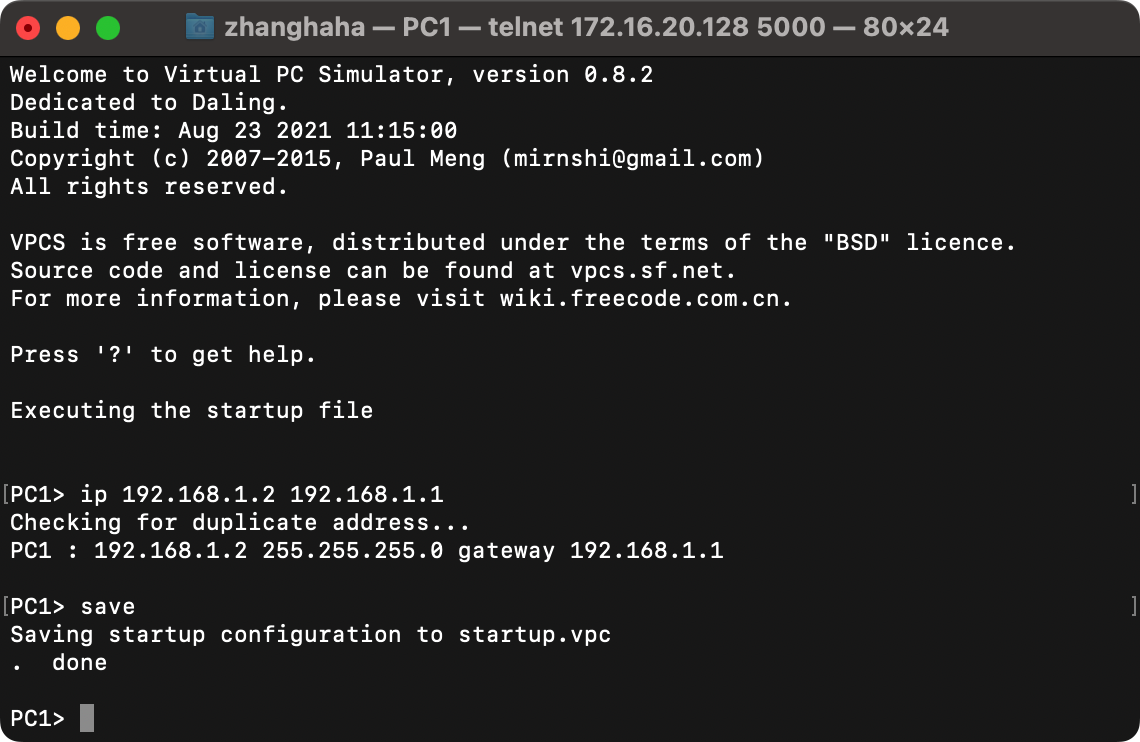
\includegraphics[width=12cm]{figure/PC1.png}
\caption{PC1}
\label{2}
\end{figure}

\begin{figure}[htb!]
  \centering
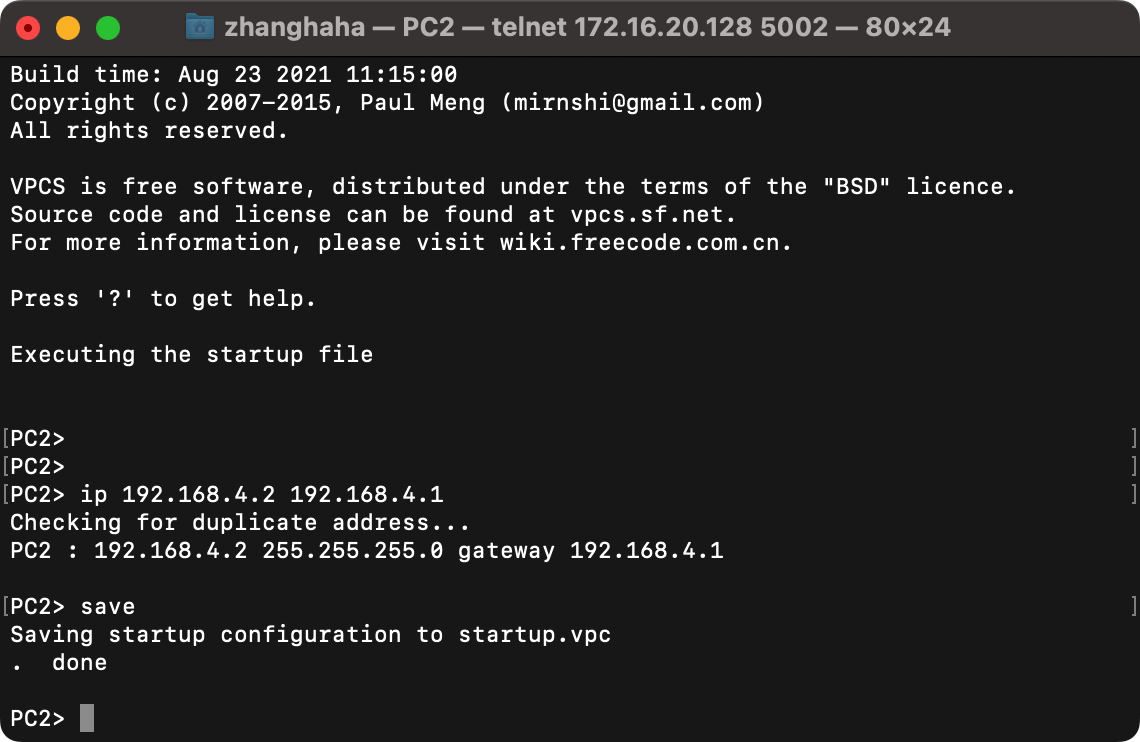
\includegraphics[width=12cm]{figure/PC2.png}
\caption{PC2}
\label{3}
\end{figure}

\subsection{路由器命名}
为路由器 RT1、RT2、RT3 分别设置主机名zhangyizhenR1,zhangyizhenR2,zhangyizhenR3。如图\ref{4},\ref{5},\ref{6}所示。
\begin{figure}[htb!]
  \centering
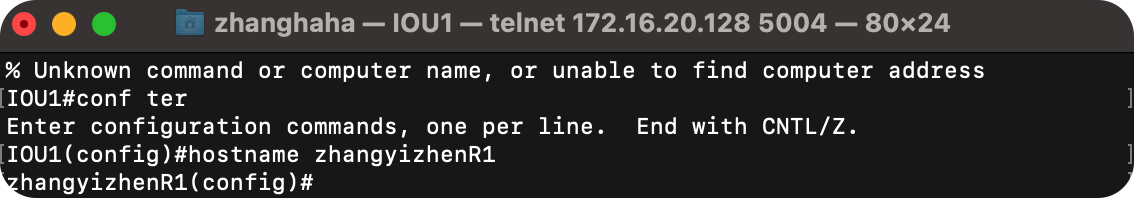
\includegraphics[width=12cm]{figure/r1.png}
\caption{zhangyizhenR1}
\label{4}
\end{figure}
\begin{figure}[htb!]
  \centering
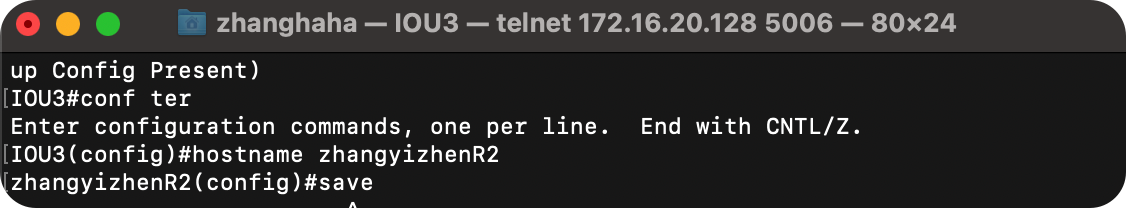
\includegraphics[width=12cm]{figure/r2.png}
\caption{zhangyizhenR2}
\label{5}
\end{figure}
\begin{figure}[htb!]
  \centering
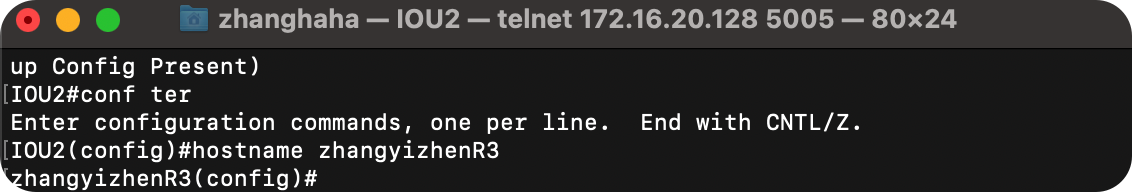
\includegraphics[width=12cm]{figure/r3.png}
\caption{zhangyizhenR3}
\label{6}
\end{figure}

\subsection{路由器配置}

\subsubsection{R1的配置}
(从左至右配置)为路由器 R1 的两个接口配置 IP 地址。配置完成后 PC1 应该可以 Ping 通 RT1 的 E0 口的地址。要求记录输入的命令和输出(截屏)。(本模拟器 R1 实际使用的接口名由实际使用的路由器型号确定,为 Ethernet0/0) 。

\begin{figure}[htb!]
  \centering
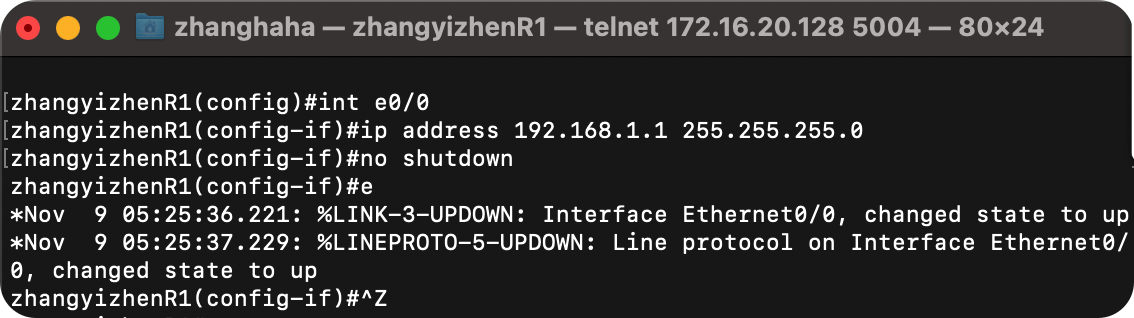
\includegraphics[width=12cm]{figure/r1e00.png}
\caption{R1 E0/0}
\label{7}
\end{figure}
\begin{figure}[htb!]
  \centering
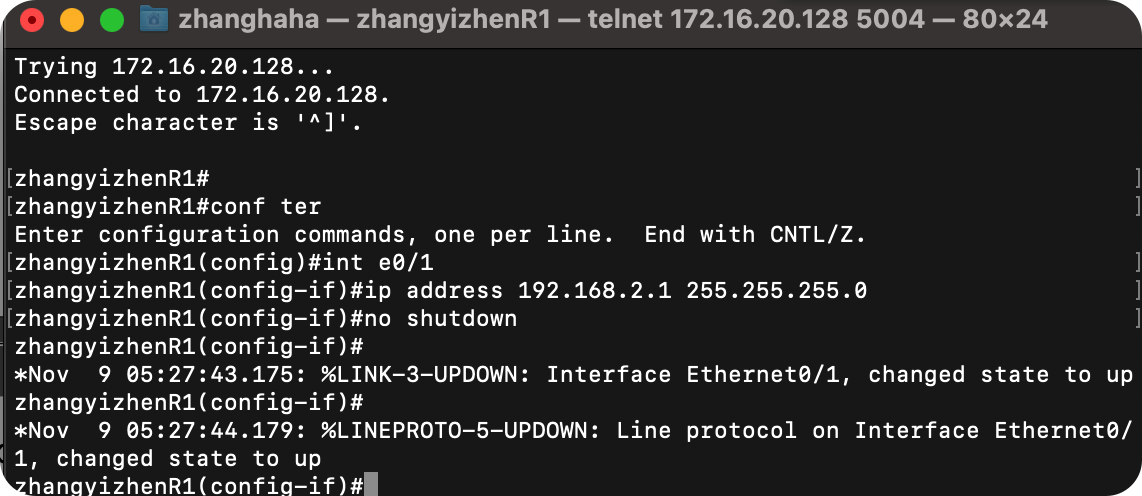
\includegraphics[width=12cm]{figure/r1e01.png}
\caption{R1 E0/1}
\label{8}
\end{figure}
\begin{figure}[htb!]
  \centering
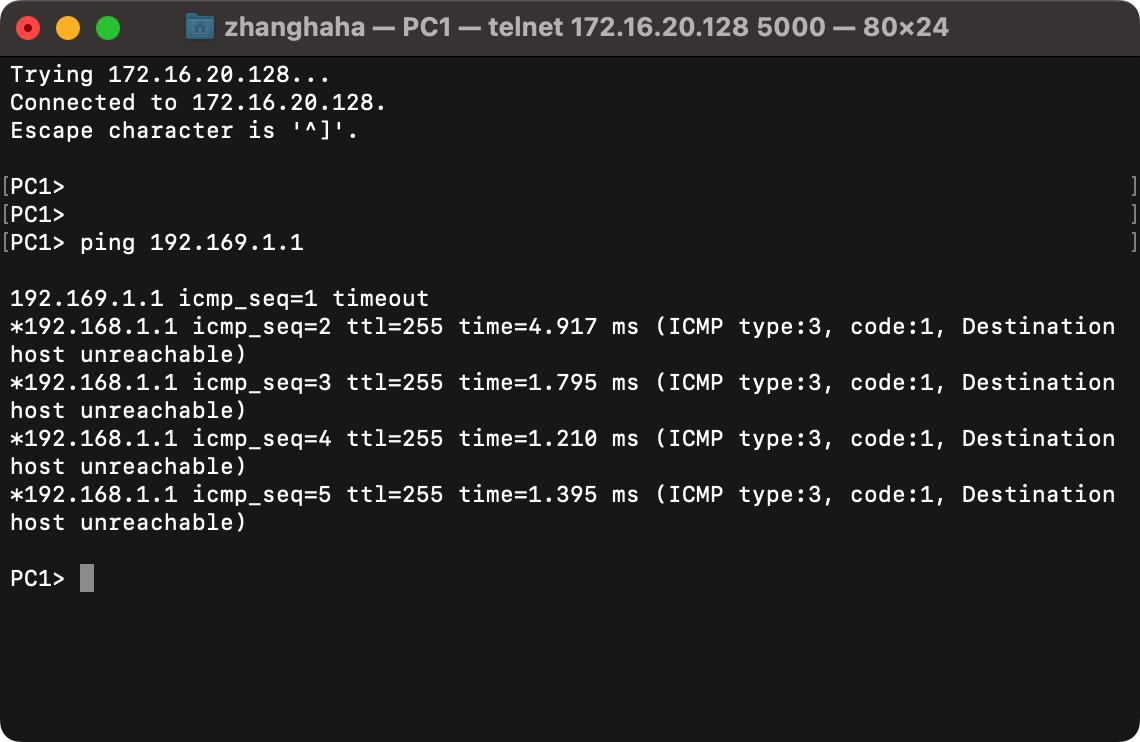
\includegraphics[width=12cm]{figure/pc1pingr1.png}
\caption{PC1 Ping R1}
\label{9}
\end{figure}

\subsubsection{R2的配置}
为路由器 R2 的 GE0、GE1 接口配置 IP 地址。配置完成后路由器 R1 和 R2 应该可以互相 Ping 通。要求记录输入的命令和输出(截屏)
\begin{figure}[htb!]
  \centering
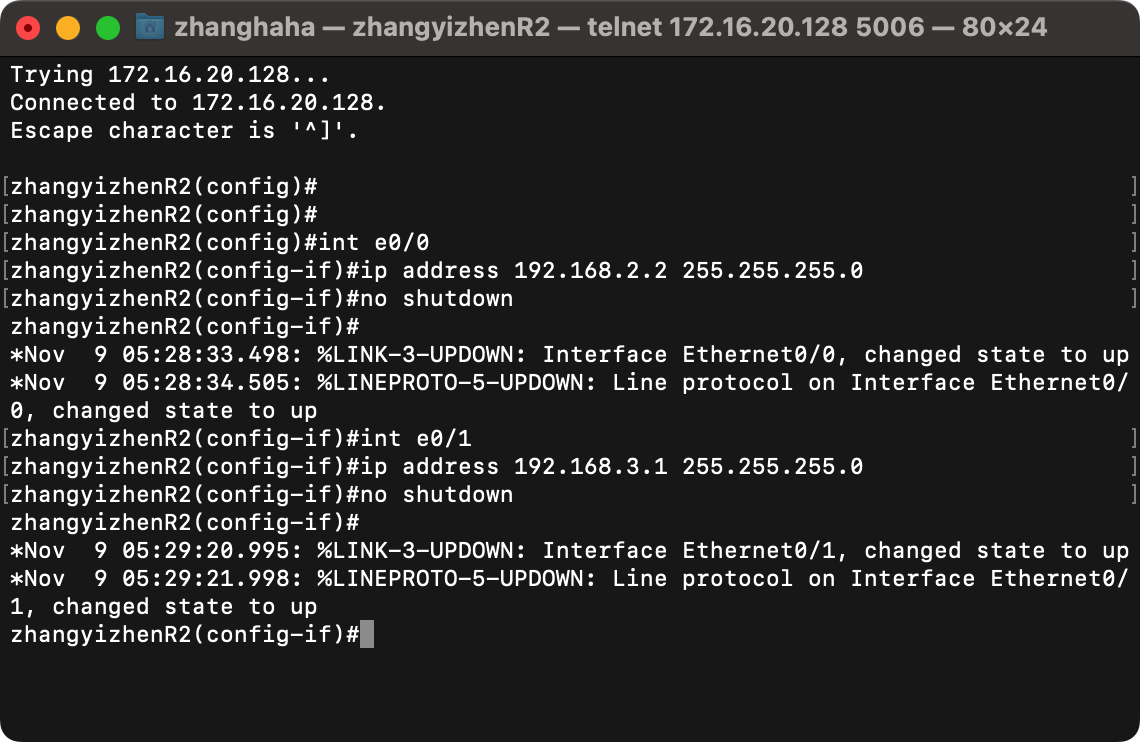
\includegraphics[width=10cm]{figure/R2e.png}
\caption{R2 E0/0\&1}
\label{10}
\end{figure}
\begin{figure}[htb!]
  \centering
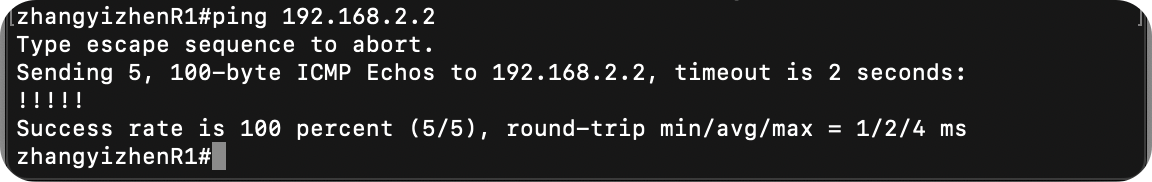
\includegraphics[width=10cm]{figure/R1pingR2.png}
\caption{R1 ping R2}
\label{11}
\end{figure}


\subsubsection{R3的配置}
为路由器 R3 的 GE0、GE1 接口配置 IP 地址。配置完成后,直连路由应可相互 Ping 通,如 PC2 应可 Ping 通 R3 的 GE1 口的地址。
\begin{figure}[htb!]
  \centering
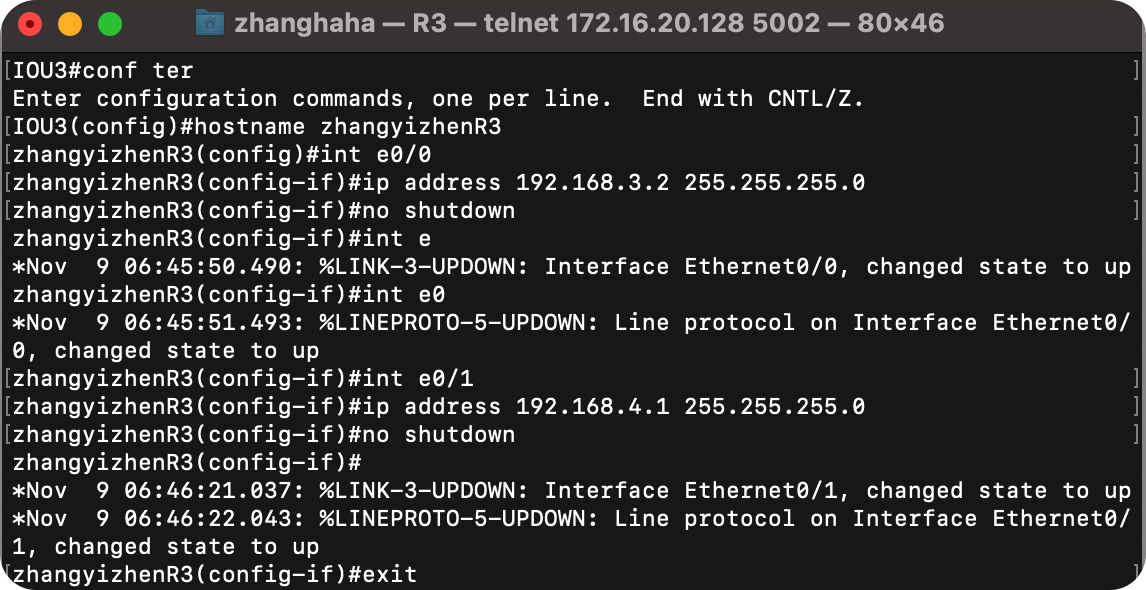
\includegraphics[width=10cm]{figure/R3e.png}
\caption{R3 E0/0\&1}
\label{12}
\end{figure}

PC2 可以 Ping 通 R3 的 192.168.4.1 地址
\begin{figure}[htb!]
  \centering
\includegraphics[width=10cm]{figure/PC2pingR3.png}
\caption{PC2 ping R3}
\label{13}
\end{figure}

\subsection{静态路由配置}
为三个路由器分别从左至右配置静态路由。如图\ref{14},\ref{15},\ref{16}所示。

\begin{figure}[htb!]
  \centering
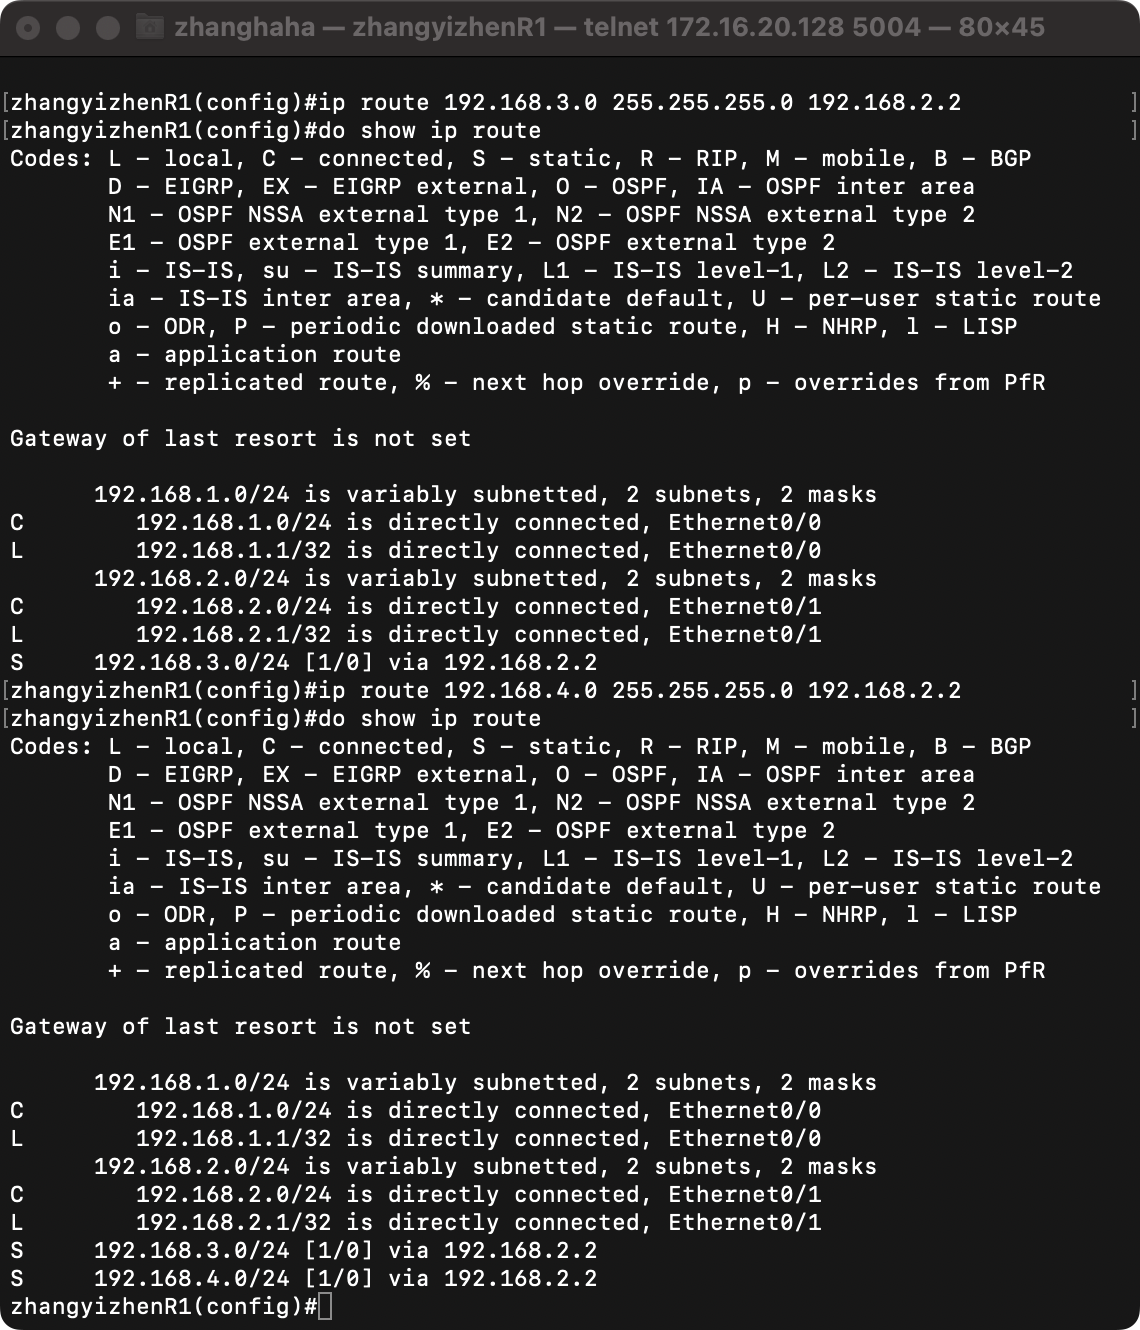
\includegraphics[width=10cm]{figure/R1s.png}
\caption{Static R1}
\label{14}
\end{figure}

\begin{figure}[htb!]
  \centering
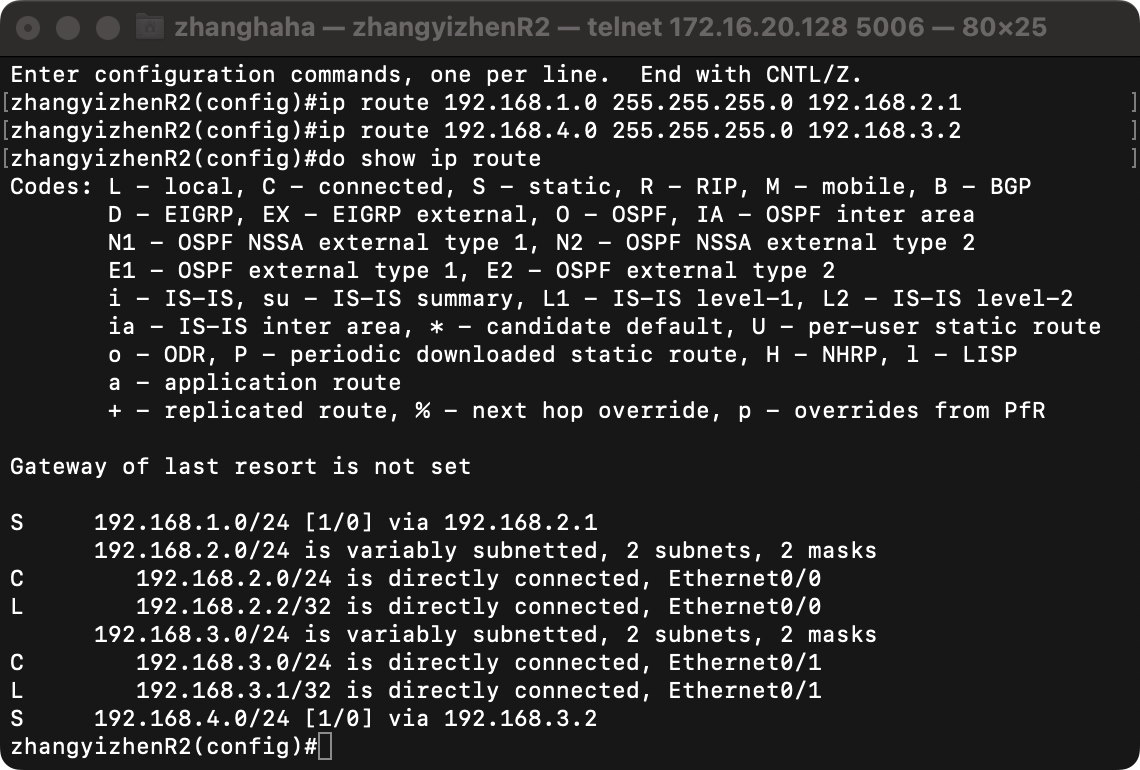
\includegraphics[width=10cm]{figure/R2s.png}
\caption{Static R2}
\label{15}
\end{figure}

\begin{figure}[htb!]
  \centering
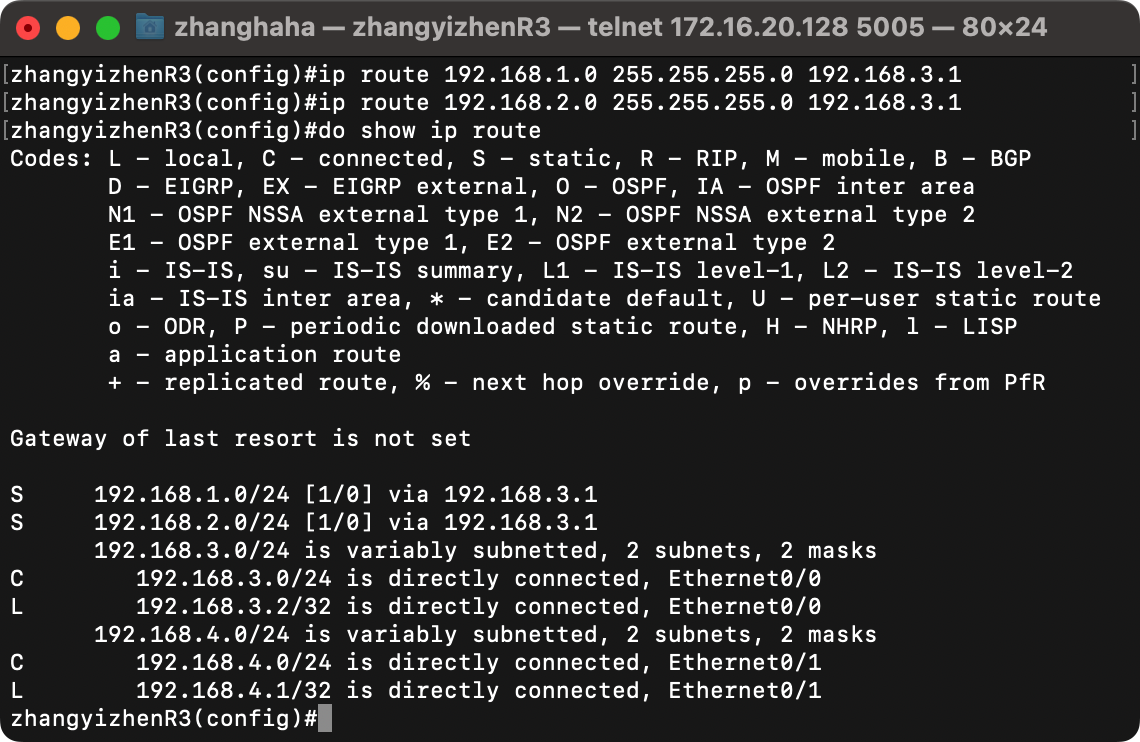
\includegraphics[width=10cm]{figure/R3s.png}
\caption{Static R3}
\label{16}
\end{figure}


\subsection{PC之间互ping}
如配置正确,此时网络收敛,则任何两点之间(含非直连)均可 ping 通,验证,如 PC1 和 PC2 可以 ping 通。分别使用 ping 命令和 traceRT 命令来验证, 解释结果显示。要求记录输入 的命令和输出(截屏)。
如图\ref{17}所示,PC2 ping PC1;如图\ref{18}所示,PC1 trace PC2。
\begin{figure}[htb!]
  \centering
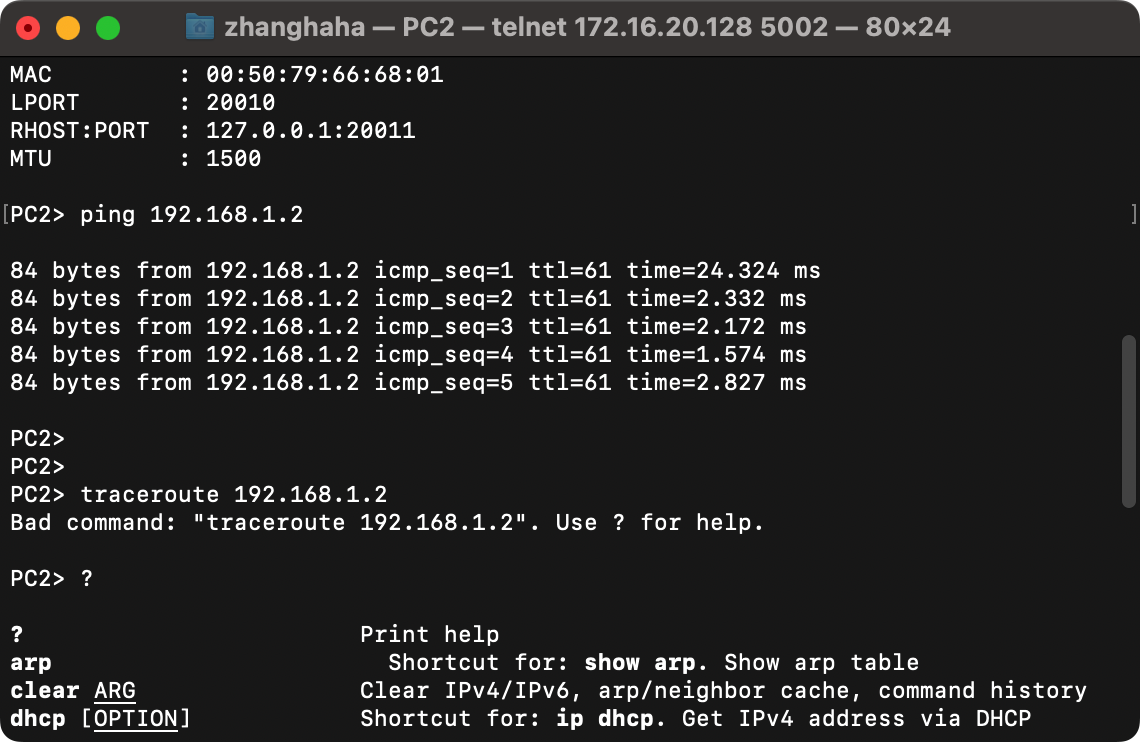
\includegraphics[width=10cm]{figure/pc2pingpc1.png}
\caption{pc2 ping pc1}
\label{17}
\end{figure}
\begin{figure}[htb!]
  \centering
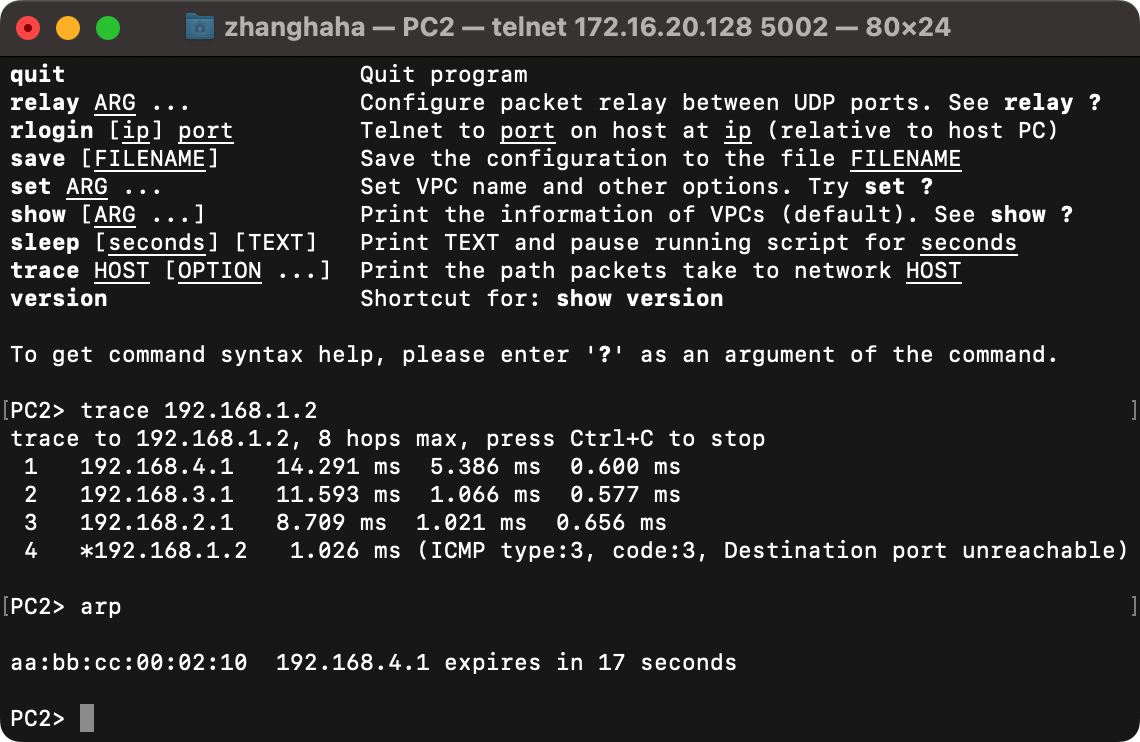
\includegraphics[width=10cm]{figure/pc2tracepc1.png}
\caption{pc2 trace pc1}
\label{18}
\end{figure}

\subsection{抓包}
在 PC1 上使用抓包工具进行抓包。首先使用 arp–d 命令清空 arp 表。再 使用 Ping 命令测试到 PC2 的连通性(192.168.4.2)。
如附件数据包所示。

% \subsubsection{网关对pc1的arp请求}
% \begin{figure}[h!]
%   \centering
%   \begin{subfigure}[b]{0.3\linewidth}
%     
\includegraphics[width=\linewidth]{figure/nankai.jpg}
%     \caption{观察PC1与Sw3之间.}
%   \end{subfigure}
%   \begin{subfigure}[b]{0.6\linewidth}
%     
\includegraphics[width=\linewidth]{figure/nankai.jpg}
%     \caption{使用WireShark抓取数据包.}
%   \end{subfigure}
%   \caption{使用WireShark抓取PC1与Sw3之间的数据包.}
%   \label{fig:128}
% \end{figure}


\end{spacing}
%---------------------------------------------------------------------
%  实验3.2
%---------------------------------------------------------------------
\chapter{动态路由(RIP)
}
\setcounter{page}{1}
\begin{spacing}{1.5}
\songti\zihao{-4}

\section{实验目的}
理解动态路由协议 RIP 的工作原理;掌握采用动态路由协议 RIP 进行网络设计的基本原则和方法。

\section{RIP协议}

RIP 是一种基于距离向量的路由选择协议,它使用跳数(Hop Count)作为度量值来衡量到达目的地址的距离。直接相连的路由器跳数为 1。跳数最多为 15,超过则表示不可达。RIP 每隔30秒和相邻路由器交换自己的路由表,经过若干次交换之后,所有路由器最终会知道到达本自治系统中任何一个网络的最短距离和下一跳路由器地址。

下例说明RIP协议是如何工作:假设我们有两条从源(R1)到目的地(R7)的路径。RIP协议将选择具有较少跳数的Route2。

Route1:R1-R2-R4-R6-R7

Route2:R1-R3-R5-R7


\subsection{RIP路由更新规则}

对地址为 X 的相邻路由器发来的 RIP 报文,先修改报文中的所有项目,把下一跳字段中的地址改为 X,并把所有的距离字段加 1;

对修改后的 RIP 报文中的每一个项目,进行以下步骤:

若原来的路由表中没有目的网络 N,则把该项目添加到路由表中;

否则:若下一跳路由器地址是 X,则把收到的项目替换原来路由表中的项目;否则:若收到的项目中的距离 d 小于路由表中的距离,则进行更新(例如原始路由表项为 Net2, 5, P,新表项为 Net2, 4, X,则更新);否则什么也不做。

若 3 分钟还没有收到相邻路由器的更新路由表,则把该相邻路由器标为不可达,即把距离置为 16。

\subsection{RIP优缺点}

RIP非常适合小型网络,它易于理解和配置,同时几乎所有路由器都支持它。但是 RIP的跳数限制为15,超出该距离则无法访问,限制了网络的规模。
RIP网络收敛速度非常慢,当网络出现故障时,要经过比较长的时间才能将此消息传送到所有路由器。由于RIP中的任何路由更新都会占用大量带宽,因此关键IT流程的资源受到限制。
RIP不支持同一路由上的多条路径,这可能会产生更多的路由环路。在使用固定跳数指标选择最佳路由时,RIP在基于实时数据比较路由时无法工作。

\section{实验步骤}
其他步骤与实验3.1相同,只需在R1和R2上配置RIP协议即可。

在GNS3中的,RIP配置命令,如图\ref{rip}
\begin{figure}[htb!]
  \centering
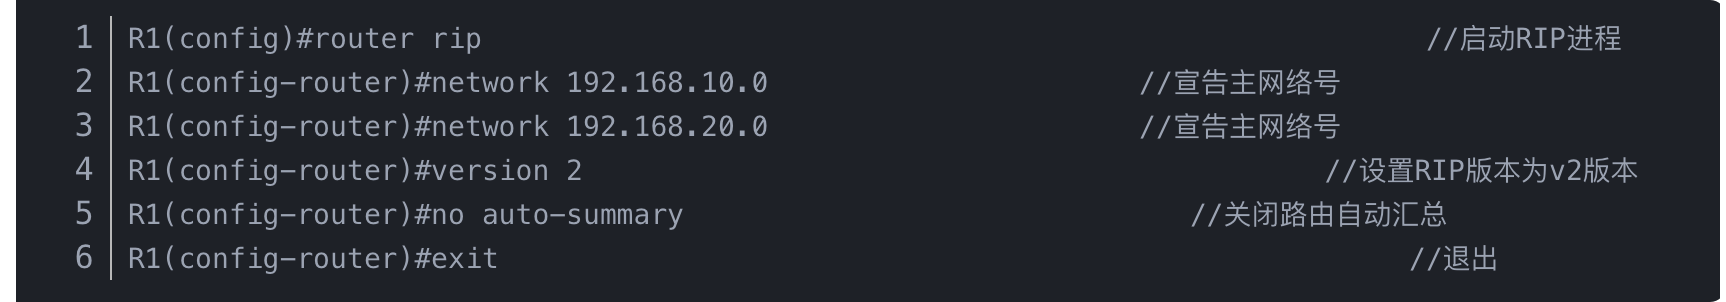
\includegraphics[width=10cm]{figure/rip.png}
  \caption{RIP协议}
  \label{rip}
\end{figure} 

\subsection{RIP协议路由器配置}
为三个路由器分别配置动态路由协议 rip(从左至右)。如图\ref{19},\ref{20},\ref{21}。
\begin{figure}[htb!]
  \centering
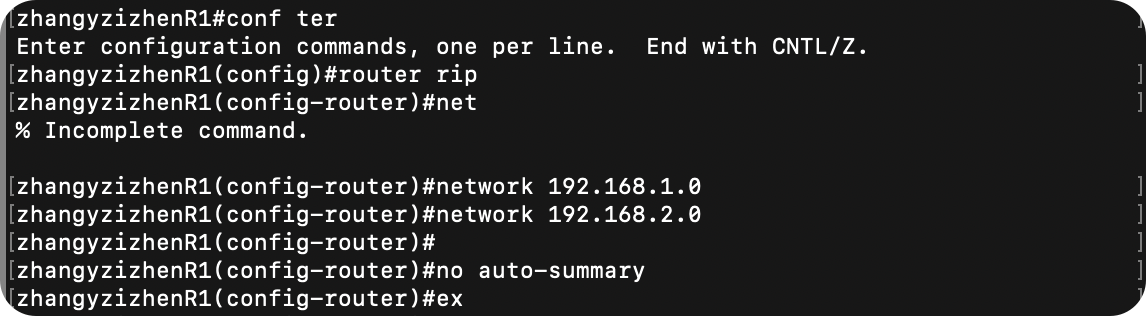
\includegraphics[width=10cm]{figure/R1rip.png}
  \caption{RIP协议R1配置}
  \label{19}
\end{figure} 
\begin{figure}[htb!]
  \centering
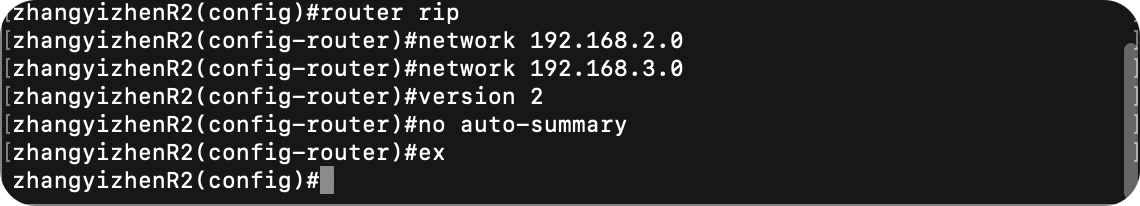
\includegraphics[width=10cm]{figure/R2rip.png}
  \caption{RIP协议R2配置}
  \label{20}
\end{figure} 
\begin{figure}[htb!]
  \centering

\includegraphics[width=10cm]{figure/R3rip.png}
  \caption{RIP协议R3配置}
  \label{21}
\end{figure}

\subsection{RIP协议配置后路由表}
如图\ref{22},\ref{23},\ref{24},是配置后的R1、R2、R3的路由表。
\begin{figure}[htb!]
  \centering
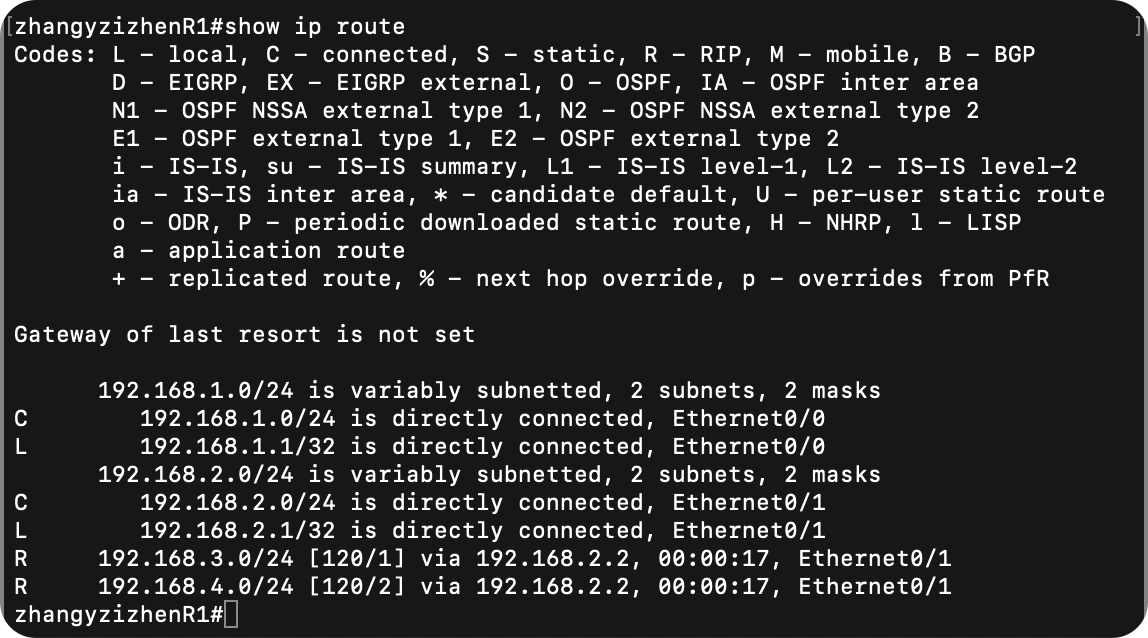
\includegraphics[width=12cm]{figure/rip-r1.png}
  \caption{RIP协议R1路由表}
  \label{22}

\end{figure}

\begin{figure}[htb!]
  \centering
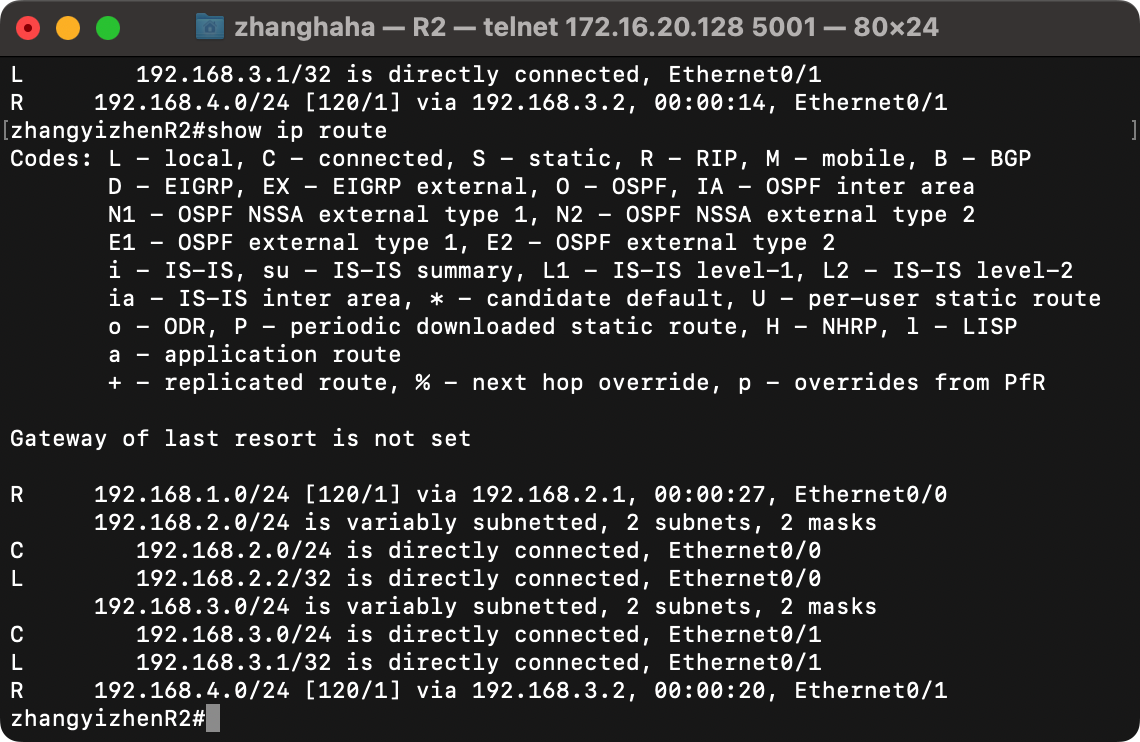
\includegraphics[width=12cm]{figure/rip-r2.png}
\caption{RIP协议R2路由表}
\label{23}
\end{figure}

\begin{figure}[htb!]
  \centering
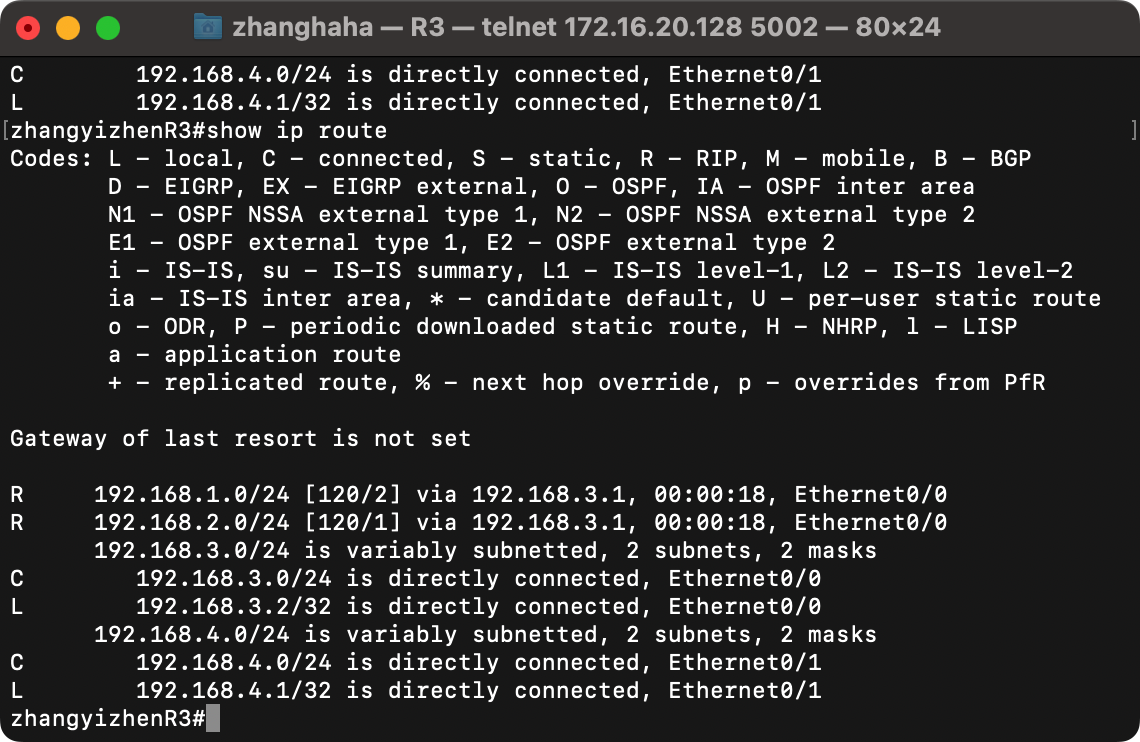
\includegraphics[width=12cm]{figure/rip-r3.png}
\caption{RIP协议R3路由表}
\label{24}
\end{figure}

\subsection{验证 PC1 和 PC2 可以 ping 通。}
如图\ref{25},附件中含有ping的数据包。
\begin{figure}[htb!]
  \centering
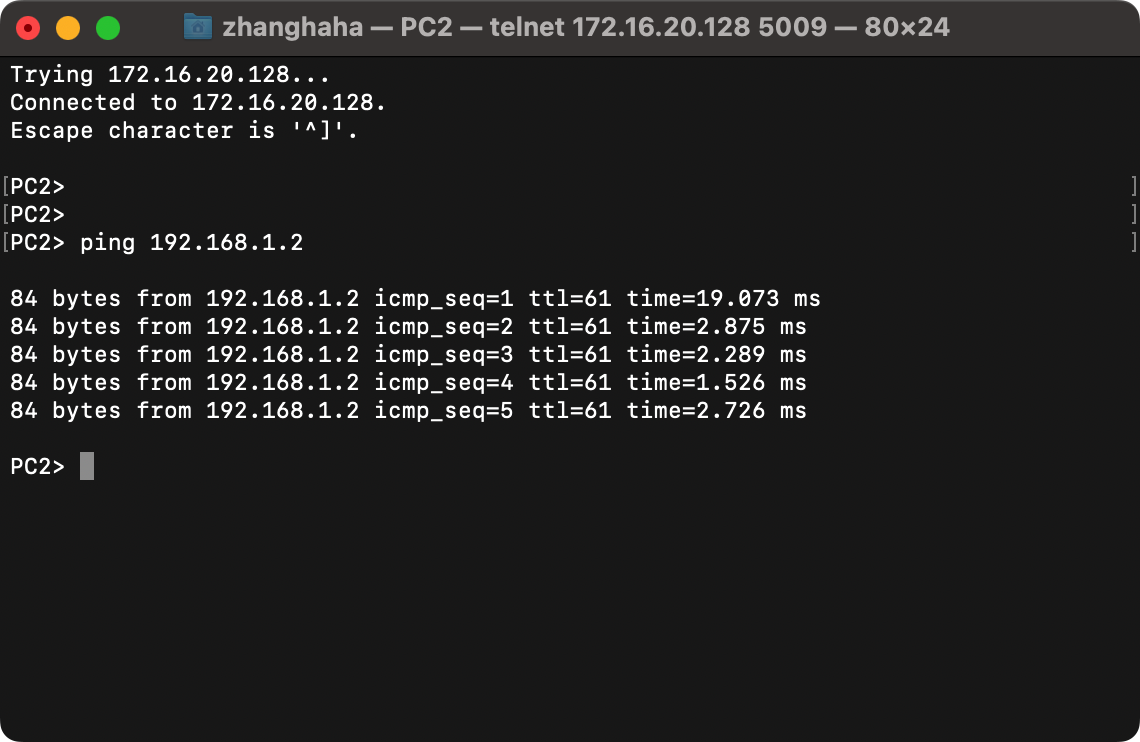
\includegraphics[width=10cm]{figure/rip ping.png}
\caption{ PIP协议 pc2 ping pc1}
\label{25}
\end{figure}


\end{spacing}

%---------------------------------------------------------------------
%  实验3.3
%---------------------------------------------------------------------
\chapter{动态路由(OSPF)
}
\setcounter{page}{1}
\begin{spacing}{1.5}
\songti\zihao{-4}

\section{实验目的}
理解动态路由协议 OSPF 的工作原理;掌握采用动态路由协议 OSPF 进行网络设计的基本原则 和方法。

\section{OSPF协议}
OSPF(开放最短路径优先 )是为了克服 RIP 的缺点而开发出来的。OSPF使用了 Dijkstra 提出的最短路径算法 SPF。使用OSPF协议需要有关复杂网络的高级知识。因此OSPF路由协议允许路由器根据传入请求计算路由。
OSPF的缺点是,当网络中添加了更多路由器时,它无法扩展。而OSPF缺乏可扩展性使其不适合在Internet上进行路由。

\subsection{OSPF工作过程}

\begin{enumerate}
\item 寻找邻居
\item 建立邻接关系
\item 链路状态信息传递
\item 计算路由
\end{enumerate}

\begin{figure}[htb!]
  \centering
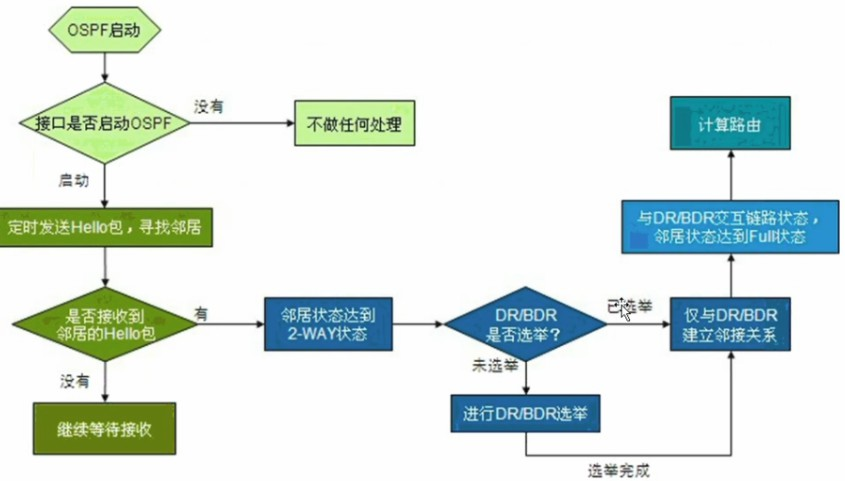
\includegraphics[width=10cm]{figure/ospfwaht.jpg}
\caption{OSPF工作过程}
\label{26}
\end{figure}

\subsection{OSPF特点}

向本自治系统中的所有路由器发送信息,这种方法是洪泛法。

发送的信息就是与相邻路由器的链路状态,链路状态包括与哪些路由器相连以及链路的度量,度量用费用、距离、时延、带宽等来表示。

只有当链路状态发生变化时,路由器才会发送信息。

所有路由器都具有全网的拓扑结构图,并且是一致的。相比于 RIP,OSPF 的更新过程收敛的很快。

\section{RIP与OSPF对比}

路由协议类型: RIP是距离矢量协议,而OSPF是链路状态协议。距离矢量协议使用跳数来确定传输路径。链路状态协议分析不同的源,如速度,成本和路径拥塞,同时识别最短路径。

路由表构造: RIP使用周围的路由器请求路由表。然后合并该信息并构造自己的路由表。该表定期发送到相邻设备,同时更新路由器的合并表。在OSPF中,路由器通过仅从相邻设备获取所需信息来合并路由表。它永远不会获得设备的整个路由表,并且路由表构造非常简单。

跳数限制: RIP最多只允许15跳,而在OSPF中没有这样的限制。

使用的算法: RIP使用距离向量算法,而OSPF使用最短路径算法Dijkstra来确定传输路由。

网络分类:在RIP中,网络分为区域和表格。在OSPF中,网络被分类为区域,子区域,自治系统和骨干区域。

复杂性级别: RIP相对简单,而OSPF则要复杂得多。

RIP与OSPF应用: RIP适用于较小的网络,因为它具有跳数限制。OSPF非常适合大型网络


\section{OSPF实验步骤}
在GNS3中的,RIP配置命令,如图\ref{ospf1},\ref{ospf2}
\begin{figure}[htb!]
  \centering
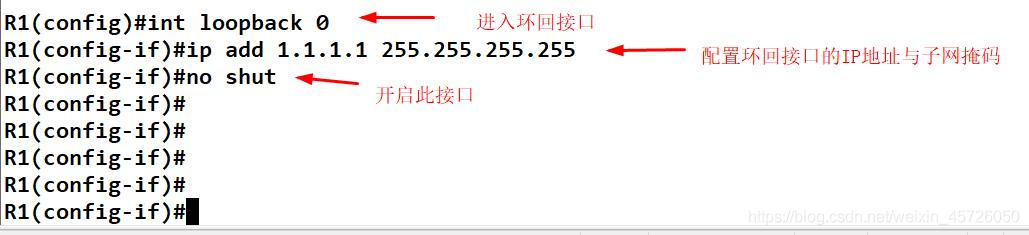
\includegraphics[width=10cm]{figure/ospf2.jpg}
  \caption{OSPF}
  \label{ospf1}
\end{figure} 

\begin{figure}[htb!]
  \centering
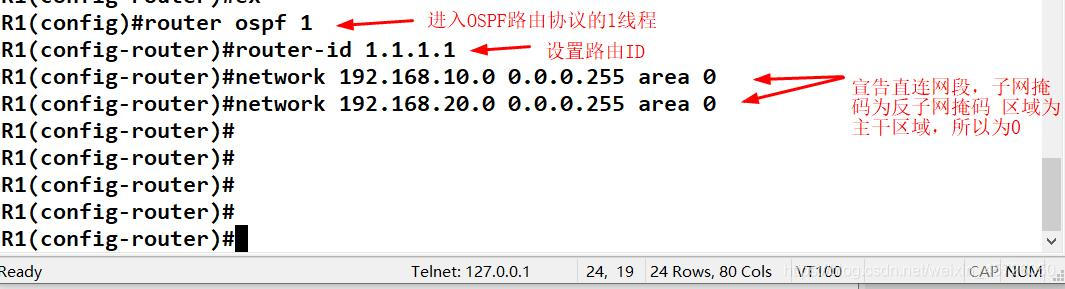
\includegraphics[width=10cm]{figure/ospf1.jpg}
  \caption{OSPF}
  \label{ospf2}
\end{figure} 

\subsection{OSPF 配置}
为 3 个路由器配置动态路由协议 ospf,首先删除原来的 rip 配置。

在GNS3中使用 no router rip删除原来的rip配置。

为 3 个路由器分别配置动态路由协议 ospf。如图\ref{27},\ref{28},\ref{29}所示。

\begin{figure}[htb!]
  \centering
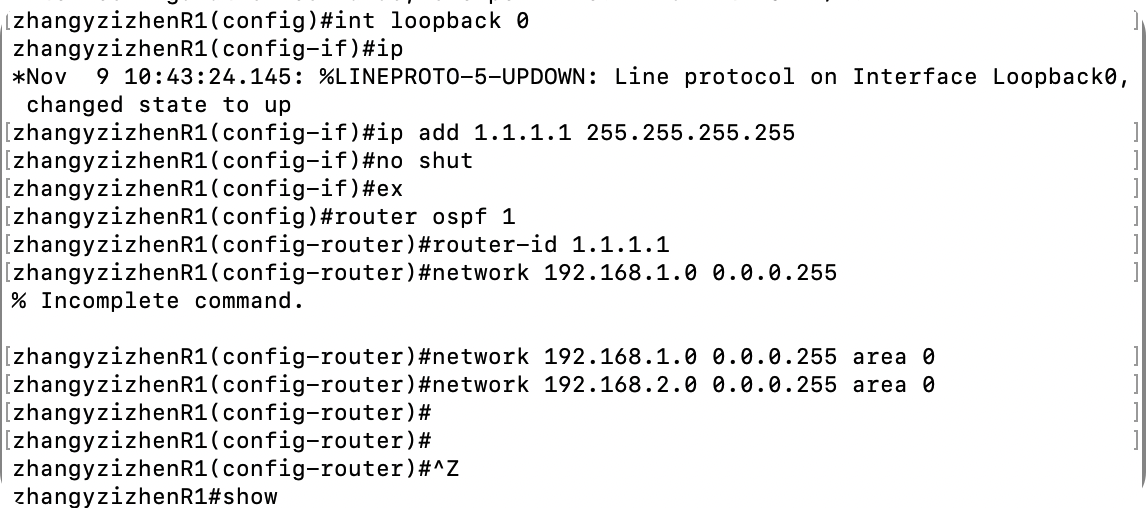
\includegraphics[width=10cm]{figure/ospf-r1.png}
  \caption{OSPF协议R1配置}
  \label{27}

\end{figure}

\begin{figure}[htb!]
  \centering
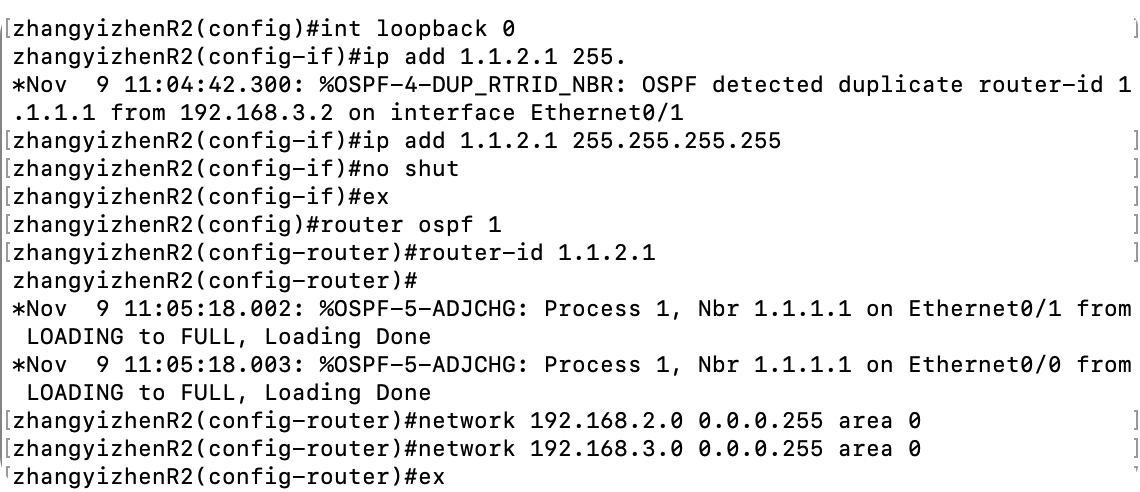
\includegraphics[width=10cm]{figure/ospf-r2.png}
\caption{OSPF协议R2配置}
\label{28}
\end{figure}

\begin{figure}[htb!]
  \centering
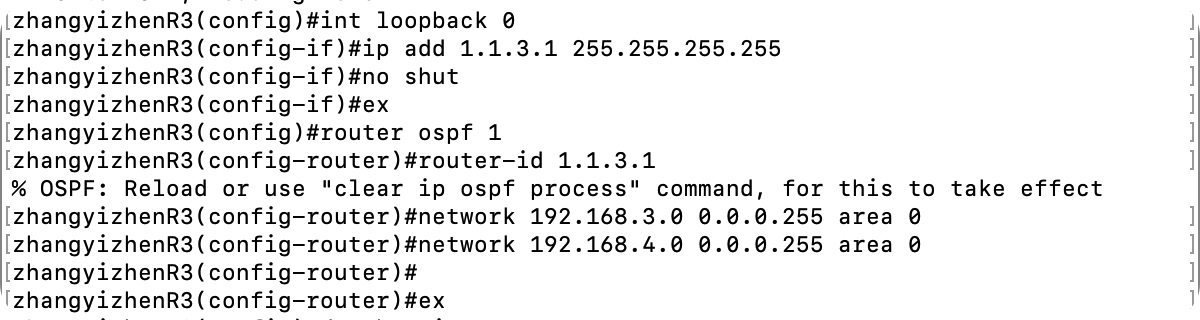
\includegraphics[width=10cm]{figure/ospf-r3.png}
\caption{ OSPF协议R3配置}
\label{29}
\end{figure}

\subsection{OSPF 配置后路由表}
配置后的路由表如图\ref{30},\ref{31},\ref{32}所示。
\begin{figure}[htb!]
  \centering
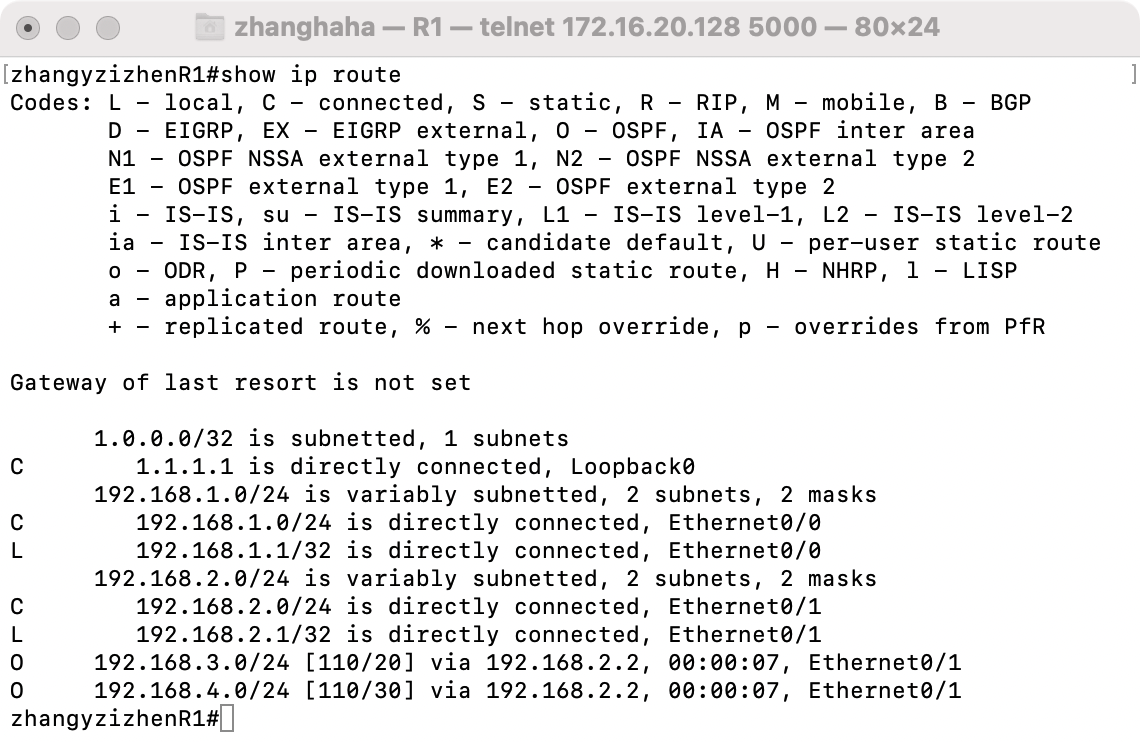
\includegraphics[width=10cm]{figure/ospf-r1-route.png}
  \caption{OSPF协议R1路由表}
  \label{30}

\end{figure}

\begin{figure}[htb!]
  \centering
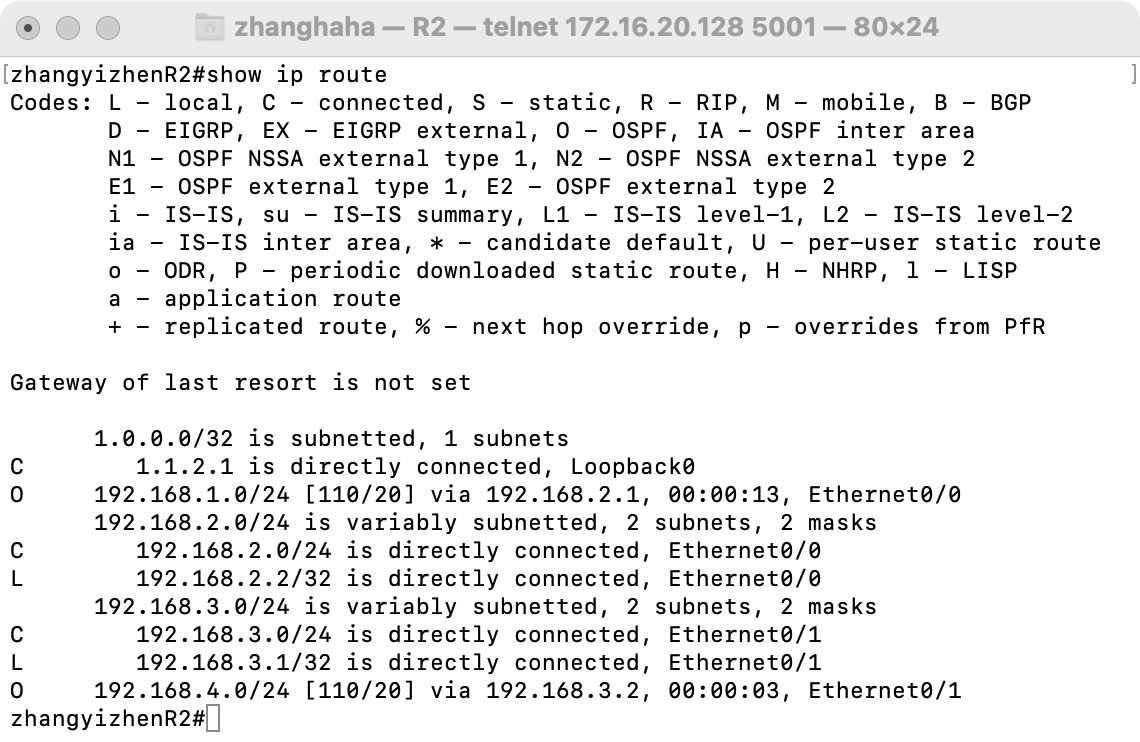
\includegraphics[width=10cm]{figure/ospf-r2-route.png}
\caption{OSPF协议R2路由表}
\label{31}
\end{figure}

\begin{figure}[htb!]
  \centering
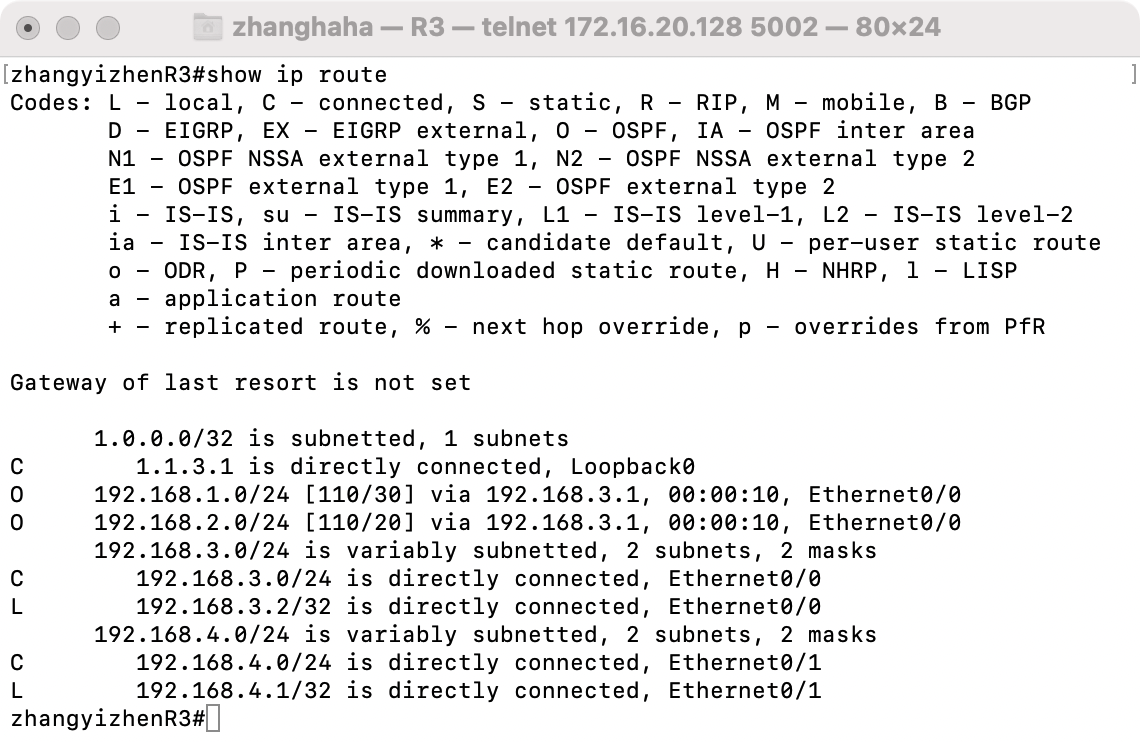
\includegraphics[width=10cm]{figure/ospf-r3-route.png}
\caption{ OSPF协议R3路由表}
\label{32}
\end{figure}

\subsection{检查是否ping通}
如图\ref{33}
\begin{figure}[htb!]
  \centering
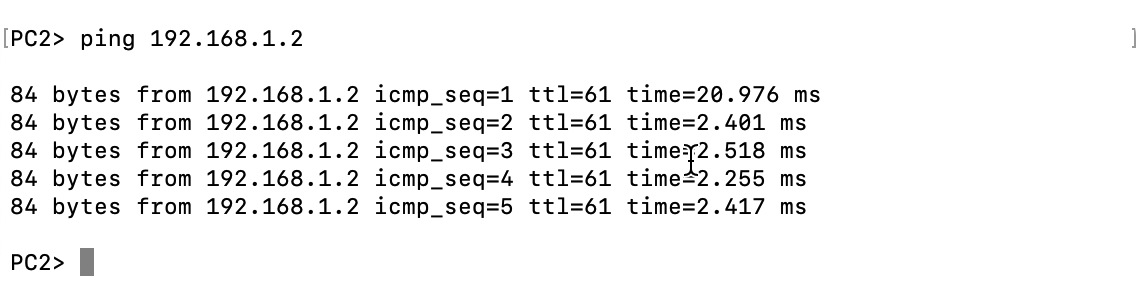
\includegraphics[width=10cm]{figure/ospf ping.png}
\caption{ OSPF协议 PC2 ping PC1}
\label{33}
\end{figure}

\section{三个实验总结}
通过本次实验,更加深入地理解了静态路由、RIP协议和OSPF协议的工作原理。虽然在一开始配置实验环境以及后续进行实验的过程中,遇到了大大小小的困难,但通过不断尝试、小心求解,最终也解决了困难。

\section{附件}
附件中另附有静态路由、RIP协议和OSPF协议的PC2 ping PC1的以及PC2 trace PC1的数据包。
\end{spacing}


\end{document}

%---------------------------------------------------------------------
%  参考文献设置
%---------------------------------------------------------------------
% \addcontentsline{toc}{chapter}{参考文献}

% \begin{thebibliography}{99}
% \songti \zihao{-4} 	
% 	\bibitem{Leslie.{1994}}
% 	Leslie Lamport. LATEX: A Document Preparation System.AddisonWesley, Reading, Massachusetts, second edition, 1994, ISBN 0-201-52983-1.
	
% 	\bibitem{Donald.{1984}}
% 	Donald E. Knuth. The TEXbook, Volume A of Computers and Typesetting,Addison Wesley, Reading, Massachusetts, second edition, 1984,ISBN 0-201-13448-9.

	
% \end{thebibliography}

%---------------------------------------------------------------------
%  附录设置
%---------------------------------------------------------------------
% \titleformat{\chapter}{\heiti\Large}{附录~\Alph{chapter}}{11pt}{\Large}
% \titlespacing{\chapter}{0pt}{*-4}{*4}

% \lstset{breaklines}                %自动将长的代码行换行排版
% \lstset{extendedchars=false}
% \lstset{language=Matlab}
% \renewcommand{\thechapter}{附录\Alph{chapter}.}
% \appendix
% \begin{appendix}
	
	

% \end{appendix}
		


